\documentclass[12pt,a4paper]{article}
\usepackage{german}
\usepackage[utf8]{inputenc}
\usepackage[T1]{fontenc}
\usepackage{ae}
\usepackage{amssymb}
\usepackage{ifthen}
\ifx\pdfoutput\undefined
\usepackage[dvips]{graphicx}
\else
\usepackage[pdftex]{graphicx}
\pdfcompresslevel=9
\pdfpageheight=297mm
\pdfpagewidth=210mm
\usepackage{color}
\usepackage{hyperref}

\definecolor{uniblue}{rgb}{0, 0.2, 0.4}

\newcommand{\cmark}[1]{{\color{uniblue} \textbf{#1}}}


\hypersetup{
colorlinks=true,
pdfpagemode=UseNone,
pdfstartview=FitH,
pdfview=FitH,
urlcolor=uniblue,
linkcolor=uniblue
}
\fi
%%
\errorcontextlines=999
%
%
\def\hs#1{\hspace*{#1cm}}
\def\spiegel#1{$\stackrel{\leftarrow}{#1}$}
\def\mspiegel#1{\stackrel{\leftarrow}{#1}}
\def\ei#1{$\ \stackrel{(#1)}{=}\ $}
\def\mei#1{\ \stackrel{(#1)}{=}\ }
\def\als{~~~$\simeq$~~~}
\def\ab{$\stackrel{uses}{\longrightarrow}\ $}
%
%
\setlength{\textwidth}{175mm}
\setlength{\oddsidemargin}{0mm}
\setlength{\evensidemargin}{0mm}
\setlength{\topmargin}{0mm}
\setlength{\textheight}{252mm}
\setlength{\voffset}{-2.4cm}
\setlength{\hoffset}{-1.2cm}
\parskip1ex
\parindent0cm
%%
\def\rand#1{\marginpar{\tiny #1}}
\def\co#1{$\overline{\mbox{#1}}$}
\def\mco#1{\overline{\mbox{#1}}}         
\def\rhd{\vartriangleright}
\def\mouver{\vartriangleright\ }
\def\ouver{$\vartriangleright\ $}
\def\folgt{$\ \Longrightarrow\ $}
\def\gdw{$\ \Longleftrightarrow\ $}
\def\rhd{$\vartriangleright$}
\def\lhd{$\vartriangleleft$}
\def\brhd{$\blacktriangleright$}
\def\blhd{$\blacktriangleleft$}
\def\bst{$\bigstar$}
\def\ost{$\circledast$}
%%%
\def\err#1{$error_{#1}$}
\def\merr#1{error_{#1}}
%
\def\tsig{$T_{SIG}$}
%
\def\mt{$\times\ $}
\def\pot#1{{\Large $\wp$}(#1)}
\def\mpotf#1{{\Large \wp_{fin}}(#1)}
\def\ab{$\stackrel{uses}{\longrightarrow}\ $}
\def\wird{~{\tt ==>}~}
\def\move{~\vdash~}
\def\mv#1{~\stackrel{#1}{\vdash}~}
\def\moves{~\stackrel{*}{\vdash}~}
\def\movep{~\stackrel{+}{\vdash}~}
\def\regel{\ \longrightarrow\ }
\def\wirdm{\ \Longrightarrow\ }
\def\wirds{~\stackrel{*}{\Longrightarrow}~}
\def\alt{\ \vert\ }
%
%
\def\ww{{\tt \#t$\ $}}
\def\ff{{\tt \#f$\ $}}
\def\mww{\mbox{\tt \#t}}
\def\mff{\mbox{\tt \#f}}
%
\def\bool{I\hskip -1.6pt B$\ $}
\def\mbool{\rm I\hskip -1.6pt B}
%
\def\pot#1{{\Large $\wp$}(#1)}
\def\mrea{\rm I\hskip -1.6pt R}
\def\mnat{\rm I\hskip -1.6pt N}
\def\mnato{\rm I\hskip -1.6pt N_0}
\def\rea{I\hskip -1.6pt R$\ $}
\def\nat{I\hskip -1.6pt N$\ $}
\def\nato{I\hskip -1.6pt N_0$\ $}
\def\aus{$ \in\ $}
\def\bull{\vrule height .9ex width .8ex depth -.1ex }
\def\gdw{:$\Longleftrightarrow$}
\def\folgt{$\ \Longrightarrow\ $}
%
\def\se{$\ \bullet\ \ $}
\def\pa{$\ \parallel\ \ $}
\def\async{$\ \equiv\hskip -6pt\equiv\hskip -3pt\gg\ \ $}
\def\sync{$\ \bowtie\hskip -6pt\rhd\ \ $}
\def\nix{$\ \infty\ $}
\def\ka{$\cal K$}
\def\seperate{\hrule\vskip 2pt\hrule\vskip 2pt\hrule}
%
\def\seperate{\hrule\vskip 2pt\hrule\vskip 2pt\hrule}
%
\newcounter{beispiel}
\newenvironment{bsp}[2]{\label{#1}\addtocounter{beispiel}{1} \vskip 8pt
\seperate \vskip 6pt
{\bf Beispiel \thechapter.\thebeispiel:} ({\em #2}) \vskip -3pt }
{\vskip 6pt
\seperate \vskip 5pt}
%
\def\strich{\begin{center} \rule{7cm}{2pt} \end{center}}
%
\newenvironment{remark}{\begin{description}\item {\bf Bemerkung:} }
{ \end{description}}
%
% ***************************************************************
\def\eg#1{eg(#1)}
\def\ag#1{ag(#1)}
\def\bs{\vskip 0.7cm}
%
%
\newcommand{\bildw}[4]{
  \begin{figure}[htb]
    \begin{center}
      \includegraphics[width=#4 cm]{images/#2}
      \caption{#3}
      \label{#1}
    \end{center}
  \end{figure}
}
%
%
\newcommand{\bildh}[4]{
  \begin{figure}[hbt]
    \begin{center}
      \includegraphics[height=#4 cm]{images/#2}
      \caption{#3}
      \label{#1}
    \end{center}    
  \end{figure}
}
%
%
\newcommand{\bild}[3]{
  \begin{figure}[hbt]
    \begin{center}
      \includegraphics[width=\textwidth]{#2}
      \caption{#3}
      \label{#1}
    \end{center}    
 \end{figure}
}
%
%
\newcommand{\atitle}{
  \begin{center}
    \begin{minipage}[t]{16cm}
      \begin{minipage}{3cm}
        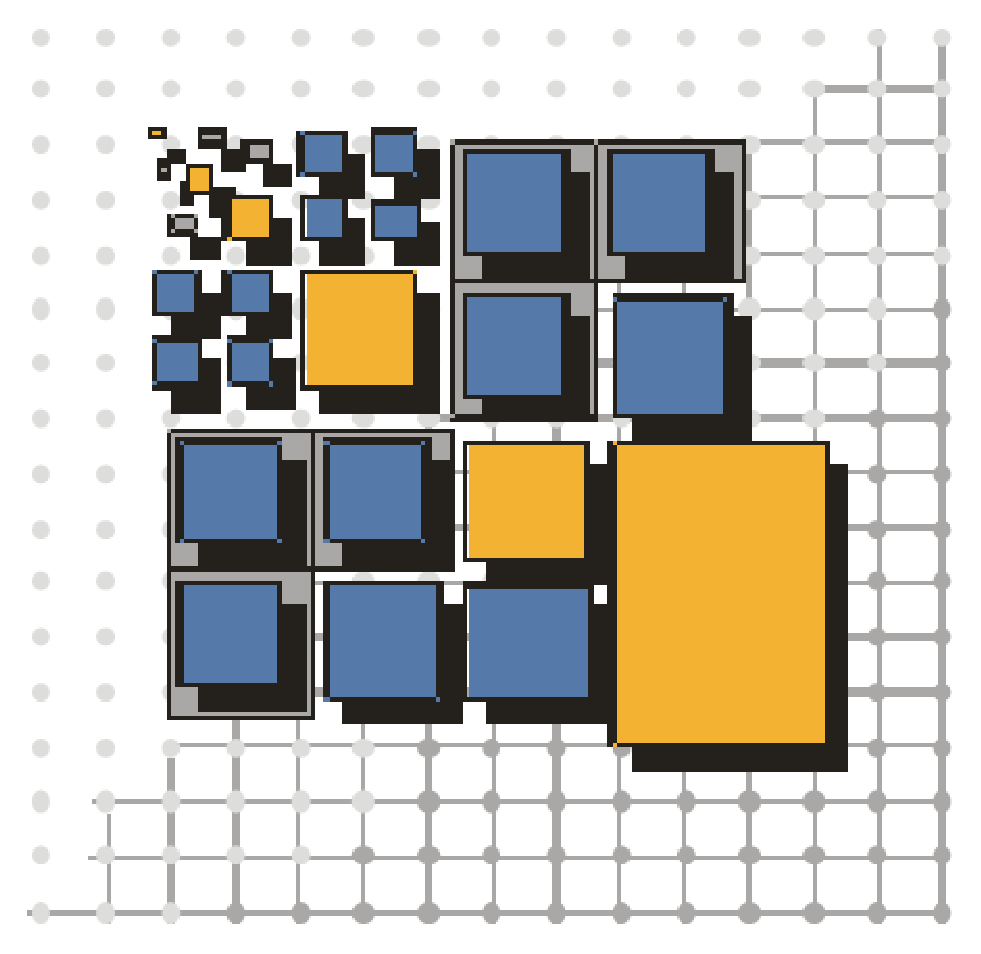
\includegraphics[height=26mm]{images/vs-logo}
      \end{minipage}
      \hfill
      \begin{minipage}{9cm}
        \centering
        {\small University of Bamberg\\}
        {\Large Distributed Systems Group\\}
			 \vspace{0.3cm}
      \end{minipage}
      \hfill
      \begin{minipage}{3cm}
        
\includegraphics[height=26mm]{images/uni}
      \end{minipage}
    \end{minipage}\\[7ex]
  \end{center}
  \ifx\pdfoutput\undefined
  \else
  \hypersetup{
    pdfauthor={Distributed Systems Group},
    pdfsubject={Richtlinien zur Erstellung von Seminar- und Abschlussarbeiten},
    pdftitle={Richtlinien zur Erstellung von Seminar- und Abschlussarbeiten}
  }
  \fi
}
%
%
\newcommand{\cci}{\\[-6ex]}
\newcommand{\cc}{\\[-4.5ex]}
%
%
\newcounter{LAufgabe}
\newenvironment{LAufgabe}{
  \addtocounter{LAufgabe}{
    \large\sc L\"osungsvorschlag  zu Aufgabe
    \theLAufgabe\\[1ex]
  }
}
{\vspace{0.5ex}}
%
%
\newcounter{Aufgabe}
\newenvironment{Aufgabe}{
  \addtocounter{Aufgabe}{1}{
%    \large\sc Aufgabe \theAufgabe\\[1ex]
  }
}
{\vspace{0.5ex}}
%
%
\newcommand{\No}{\N_0}
\newcommand{\N}{\mathbb{N}}
\newcommand{\R}{\mathbb{R}}
\newcommand{\Z}{\mathbb{Z}}
\newcommand{\Q}{\mathbb{Q}}
%
\newcommand{\Ltitel}[1]{
{~\\[-2.5cm] 
\begin{center}
\Large\sc Informatik I~$\cdot$~
{\LARGE\sc \"Ubungsblatt #1}~$\cdot$~WiSe 1997/98
\end{center}~\\[-52pt]}{\LARGE\sc
~\begin{center}
L\"osungsvorschl\"age\\[4ex]
\end{center}
}}
%
%
\newcommand{\link}[2]{
  \ifx\pdfoutput\undefined
  #1 (#2)
  \else
  \href{#2}{#1}
  \fi  
}

%%% Local Variables: 
%%% mode: latex
%%% TeX-master: "ueb1"
%%% TeX-master: t
%%% TeX-master: t
%%% End: 

%
\begin{document}
% Vorlesung, Blatt-#, Autor, Key-Words (mit Kommata)
\atitle
%
\begin{center}
{\bf\huge Guidelines for writing seminar-, bachelor-, and mastertheses}

{\it April 2019}
\end{center}
%
\section{Structure of seminar-, bachelor- and mastertheses}
%

For writing theses, it is mandatory to use the DSG templates provided in the general VC course\footnote{\url{https://vc.uni-bamberg.de/moodle/course/view.php?id=2139}}. They already include the title page, lists of content, and formatting options.

\subsection{Lists of content}

At the beginning of a thesis, right after the title page, there are the following lists:

\begin{itemize}
	\item Contents
	\item List of Figures
	\item List of Tables
	\item Listings
	\item Abbreviations.
\end{itemize}

The list of contents, list of figures, list of tables, and list of listings are created automatically in all templates when the designated formatting options for figures and tables are used.\footnote{Check the documentation inside the Word or LaTeX documents}. 
The list of abbreviations includes all abbreviations used in the thesis, sorted alphabetically, and no more.
Excluded from the list of abbreviations are commonly known abbreviations, such as 'e.g.' or 'i.e.'
Abbreviations have to be written out when they are first used and the abbreviation has to be put in brackets after the written out version.

\textit{Example}: In the text: "`...for this, the \textit{Java Development Kit} (JDK) was used..."'\\
Entry in the list of abbreviations: -- "`\textit{JDK} \hspace{10pt} Java Development Kit"'.

Lists which are not needed, have to be removed before the submission of the thesis.
After the lists, follows the main part of the thesis.

\subsection{Main part}
The main part includes the actual work.
You should coordinate the concrete structure with your supervisor.
The following can serve as a reference:\\
The main part begins with the introduction which outlines the topic and motivates the thesis.
After the introduction, a short overview of the proceeding and the following sections is given, to provide the reader with a 'big picture' of the work.
The following sections then present the actual work.
The thesis is ended with a summary which presents the main conclusions and evaluates the work as a whole. \footnote{For example, a comparison of advantages and disadvantages of the used methods or self-developed solutions, etc.}. 
Furthermore, the summary should provide an outlook on possible future work on the topic of the thesis.

\subsection{Citations and Bibliography}

A thesis is based on \textit{thoroughly} researched literature sources which have to be referenced.
The bibliography may therefore contain the following types of literature:
\begin{itemize}
	\item (Text-)books,
	\item Articles from scientific journals,
	\item Proceedings of Conferences and Workshops,
	\item Technical reports
	\item and Standards
\end{itemize}

Sources should be described as detailed as possible, in order to identify and retrieve them.
In general, the author and title should always be given.
Further details depend on the specific type of literature: 

\begin{itemize}
	\item Books: Author, Title, Edition, Publisher, Date\footnote{at least the year, if possible also the month}
	\item Journal articles: Author, Title, Name of the journal, Volume, Number, Pages
	\item Proceedings of conferences and workshops: Author, Title, Name of the conference, Place, Date, Pages
	\item Technical reports: Author, Organization (e.g. University), Title, Date
	\item Standards: Name of the issuing organization Name (without specific authors), Title, Version, Date
\end{itemize}

The bibliography must not include non-scientific sources\footnote{Notably, Web sites, Manuals, Articles from non-scientific magazines, etc.}. 
If you cite such sources, you should use a footnote instead.
Excluded from being used as a source is everything written for the same purpose (other theses) or for teaching material
If you are in doubt about a specific source, ask your supervisor.

You can cite sources with a direct or indirect citation.
This has to be marked explicitly.
A citation is direct, if a statement is used literally.
A citation is indirect, if a statement is reproduced using own words.

Direct citations have to be separated from other text by using quotations marks and the source has to referenced with its number from the bibliography with page numbers. 
Example: "`This is a literal citation from a source"' ([22] p. 231). 
If parts of text are omitted within a citation, this has to be marked with '[...]'.
If parts of text are added to improve the understandability, they have to surrounded by square brackets as well. 
Further additions to the text (e.g. underlining	or highlighting) also need to be marked as own additions.
If a citation is a word-by-word translation from a foreign language, it also counts as a direct citation and it has to be marked that it is a translation.
Indirect citations also need to be referenced with the number from the bibliography and a page number.
If the citation is based on two pages this has to be marked with f. (following).
If it is based on three to five pages, this has to marked with ff. and for citations from more than five pages this has to be marked with the concrete number of pages (E.g. p. 15--23).

\subsection{Appendix}

After the bibliography, an appendix can follow, if needed.
An appendix can include further explanations, figures, tables, etc. which provide more detailed information, but are not required to understand the thesis.
This is especially relevant for bachelor- and mastertheses, for which important parts of the source code\footnote{It is undesired to present the complete source code} or complete UML diagrams can be included in the appendix, while the main part only includes extractions from the source code or diagrams.

The last page of a thesis should include the declaration of originality (Eigenständigkeitserklärung), as required by the examination office.

\newpage
\section{Submission}

The submission of a thesis has to be made according to the rules defined in the examination regulations (Prüfungsordnung).
For theses with a practical part, the source code, UML diagrams, required libraries and the compiled software have to be added to the thesis on a disk.
In addition to the submission at the examination office, the thesis has to be given to the supervisor as a PDF file (e.g. using e-mail or a disk).

The submission of seminar theses has to be coordinated with the respective supervisor.
In general, they are submitted via Email as a PDF file on the day they are due.

\section{Grading of theses}

The grading of a thesis is based on its content and formal requirements.
Therefore, it is necessary to comply with the rules described here.
The thesis should not include great linguistic deficiencies (Spelling and grammar mistakes).
Of special importance is the correct reference of used literature sources.
If literature sources are not referenced properly, the thesis might be graded with insufficient.


\section{Notes on Microsoft Word and \LaTeX}

In the general VC-course, the chair provides templates for LaTeX as well as Microsoft Word.
For both template types, it is forbidden to change the predefined spacing and formatting.
\textbf{The DSG chair generally recommends to use the TeX/LaTeX template}, because there the creation and management of the bibliography can be done automatically with BibTeX.

More helpful information on using LaTeX can be found in the template "`dsg-seminar-with-instructions"'.
%
\end{document}